% ============================================================
% 21-bezier-quartic-makie-explained.tex
% Compile with:  pdflatex -shell-escape 21-bezier-quartic-makie-explained.tex
% The PNG must be in the same folder. Run twice for TOC.
% ============================================================

\documentclass[12pt, a4paper]{article}

\usepackage[T1]{fontenc}
\usepackage[utf8]{inputenc}
\usepackage{lmodern}
\usepackage[top=2.5cm, bottom=2.5cm, left=2.8cm, right=2.8cm]{geometry}
\usepackage{graphicx}
\usepackage{float}
\usepackage[dvipsnames]{xcolor}

\definecolor{codebg}{RGB}{248,248,248}
\definecolor{rulecolor}{RGB}{180,180,180}
\definecolor{examplebg}{RGB}{240,248,255}
\definecolor{examplerule}{RGB}{100,149,237}
\definecolor{notebg}{RGB}{255,250,230}
\definecolor{noterule}{RGB}{210,180,50}

\usepackage{minted}
\setminted[julia]{
  bgcolor=codebg, frame=leftline, framerule=1.5pt,
  rulecolor=rulecolor, linenos=false, fontsize=\small,
  breaklines=true, tabsize=4, style=friendly,
}

\usepackage{amsmath}
\usepackage{amssymb}
\usepackage{tikz}
\usetikzlibrary{shapes.geometric, arrows.meta, positioning}
\usepackage{mdframed}

\newmdenv[backgroundcolor=examplebg, linecolor=examplerule,
  linewidth=1.5pt, leftline=true, rightline=false,
  topline=false, bottomline=false,
  innerleftmargin=10pt, innerrightmargin=8pt,
  innertopmargin=6pt, innerbottommargin=6pt,
  skipabove=6pt, skipbelow=4pt]{examplebox}

\newmdenv[backgroundcolor=notebg, linecolor=noterule,
  linewidth=1.5pt, leftline=true, rightline=false,
  topline=false, bottomline=false,
  innerleftmargin=10pt, innerrightmargin=8pt,
  innertopmargin=6pt, innerbottommargin=6pt,
  skipabove=6pt, skipbelow=4pt]{notebox}

\usepackage[colorlinks=true, linkcolor=black, urlcolor=MidnightBlue]{hyperref}
\usepackage{booktabs}
\usepackage{needspace}
\usepackage{parskip}
\usepackage{titlesec}
\usepackage{fancyhdr}
\usepackage{datetime2}

\titleformat{\section}
  {\large\bfseries\color{MidnightBlue}}{\thesection.}{0.6em}{}
  [\vspace{-4pt}\rule{\linewidth}{0.4pt}]
\titleformat{\subsection}
  {\normalsize\bfseries\color{BrickRed}}{\thesubsection.}{0.5em}{}
\titleformat{\subsubsection}
  {\normalsize\bfseries}{\thesubsubsection.}{0.5em}{}

\pagestyle{fancy}
\fancyhf{}
\rhead{\textcolor{gray}{\small 21-bezier-quartic-makie-explained}}
\lhead{\textcolor{gray}{\small B\'ezier Quartic 3-D --- CairoMakie}}
\cfoot{\thepage}
\renewcommand{\headrulewidth}{0.3pt}

\newcommand{\cd}[1]{\texttt{#1}}

\title{%
  \vspace{1cm}
  {\LARGE\bfseries B\'ezier Curve: Quartic (3-D)}\\[0.4em]
  {\large CairoMakie Visualisation}\\[0.4em]
  {\large Code and Plot Explanation for Julia Beginners}\\[0.4em]
  {\normalsize\texttt{21-bezier-quartic-makie.jl}}
}
\author{E.R.\ Nurwijayadi}
\date{\DTMtoday}

\begin{document}

\maketitle
\thispagestyle{empty}

\begin{center}
\textit{Directed and curated by E.R.\ Nurwijayadi.
Code and explanations AI-generated.}
\end{center}

\begin{center}
\begin{minipage}{0.85\textwidth}
\small
This document explains \cd{21-bezier-quartic-makie.jl}.
This is the first 3-D plot in the series.
The curve is the same quartic B\'ezier (5 control points)
used throughout scripts~01--05 for algebraic computation.
New concepts: \cd{Axis3} for 3-D axes, camera angles
(\cd{elevation}, \cd{azimuth}), three-argument drawing
functions, \cd{Label} for figure-level text overlays,
and generating a highlight list with \cd{collect} + \cd{round.}.
\end{minipage}
\end{center}

\vspace{1em}\hrule\vspace{1.5em}
\tableofcontents
\newpage


% =============================================================
\needspace{8\baselineskip}
\section{The Plot}
% =============================================================

\begin{figure}[H]
  \centering
  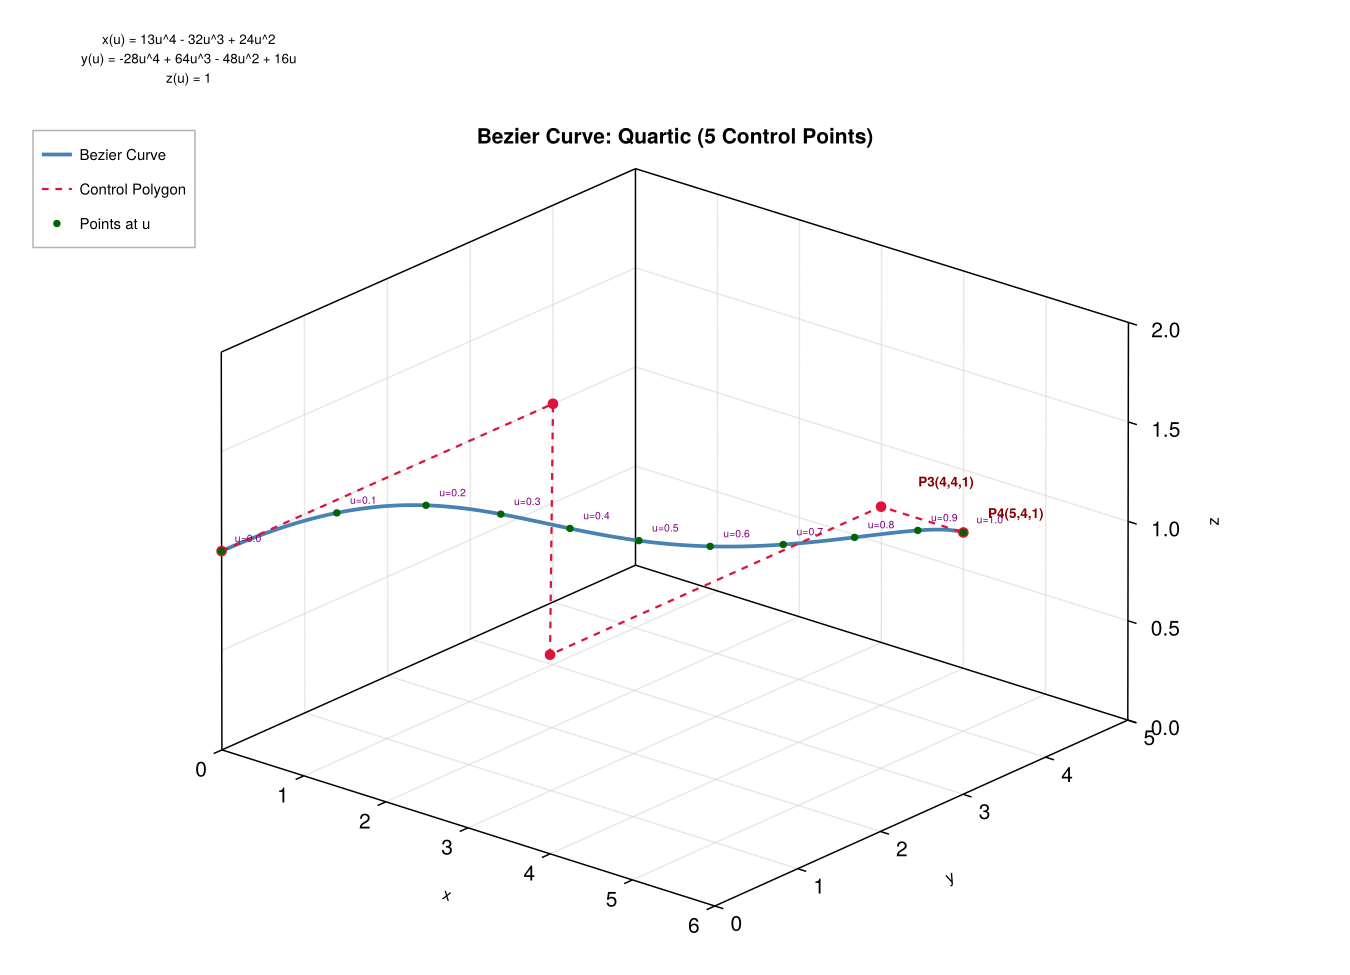
\includegraphics[width=0.95\linewidth]{21-bezier-quartic-makie.png}
  \caption{Quartic B\'ezier curve in 3-D space, with 5 control
           points and 11 highlighted curve points at
           $u = 0.0, 0.1, \ldots, 1.0$.}
  \label{fig:quartic-3d}
\end{figure}


% =============================================================
\needspace{8\baselineskip}
\section{Reading the Plot}
% =============================================================

\needspace{5\baselineskip}
\subsection{The 3-D space}

This is the same quartic B\'ezier curve computed in scripts~01--05,
now displayed in the full 3-D space $(x, y, z)$.
The five control points are:

\begin{center}
\begin{tabular}{cccc}
\toprule
Point & $x$ & $y$ & $z$ \\
\midrule
$P_0$ & 0 & 0 & 1 \\
$P_1$ & 0 & 4 & 1 \\
$P_2$ & 4 & 0 & 1 \\
$P_3$ & 4 & 4 & 1 \\
$P_4$ & 5 & 4 & 1 \\
\bottomrule
\end{tabular}
\end{center}

All five points have $z = 1$, so the curve lies entirely
in the horizontal plane $z = 1$.
In the 3-D view this appears as a flat curve hovering
above the $z = 0$ floor.

\needspace{5\baselineskip}
\subsection{Visual elements}

\textbf{Blue curve} --- the quartic B\'ezier, 300 sample points.

\textbf{Red dashed polygon} --- the control polygon connecting
$P_0 \to P_1 \to P_2 \to P_3 \to P_4$.
Notice how $P_1$ and $P_2$ are the two ``off-path'' points ---
the polygon dips below into different $y$ values and creates
the characteristic crossing pattern visible in the 3-D view.

\textbf{Green dots} --- 11 highlighted points at
$u = 0.0, 0.1, 0.2, \ldots, 1.0$,
each labelled with its $u$ value.

\textbf{Equation text (top-left)} --- the three parametric
polynomials $x(u)$, $y(u)$, $z(u)$ displayed above the plot
in monospace font.
These are the same results computed in scripts~01--05.

\needspace{5\baselineskip}
\subsection{The camera viewpoint}

The plot is rendered from a specific 3-D camera angle.
You can see the $x$ axis running left-to-right along the
bottom-front edge, the $y$ axis running right-to-back,
and the $z$ axis vertical on the right.
The viewpoint is set by \cd{elevation} and \cd{azimuth}
in the code (explained in Section~\ref{sec:axis3}).


% =============================================================
\needspace{8\baselineskip}
\section{Data and Constants}
% =============================================================

\needspace{5\baselineskip}
\subsection{Control points --- the full matrix stored directly}

\begin{minted}{julia}
const CONTROL_POINTS = [
    0.0  0.0  1.0;   # P0
    0.0  4.0  1.0;   # P1
    4.0  0.0  1.0;   # P2
    4.0  4.0  1.0;   # P3
    5.0  4.0  1.0;   # P4
]
\end{minted}

A $5 \times 3$ matrix --- five rows (one per point),
three columns ($x$, $y$, $z$).
This is the same control point data used in scripts~01--05
for algebraic computation, now stored directly as a matrix.

\needspace{5\baselineskip}
\subsection{\texttt{U\_HIGHLIGHT} --- range to vector}

\begin{minted}{julia}
const U_HIGHLIGHT = round.(collect(0.0:0.1:1.0), digits=2)
\end{minted}

This one line packs three operations:

\textbf{\cd{0.0:0.1:1.0}} --- a \textbf{range} from 0 to 1
in steps of 0.1.
In Julia, \cd{a:step:b} creates a lazy range object ---
it does not allocate memory for all the values yet.

\textbf{\cd{collect(...)}} --- converts the lazy range
into a concrete \cd{Vector\{Float64\}}:
\cd{[0.0, 0.1, 0.2, 0.3, ..., 1.0]}.

\textbf{\cd{round.(..., digits=2)}} --- applies
\cd{round(x, digits=2)} to every element using broadcast.
This is a safety measure: floating-point arithmetic can
produce values like \cd{0.30000000000000004} instead of
\cd{0.3} due to binary representation.
Rounding to 2 decimal places cleans these up.

\begin{examplebox}
\textbf{Result of \cd{U\_HIGHLIGHT}:}

\cd{[0.0, 0.1, 0.2, 0.3, 0.4, 0.5, 0.6, 0.7, 0.8, 0.9, 1.0]}

11 values. These produce the 11 green dots on the plot.
\end{examplebox}

\needspace{5\baselineskip}
\subsection{3-D offsets}

\begin{minted}{julia}
const CTRL_OFFSETS = [
    (-0.3, -0.4,  0.05),
    (-0.3,  0.3,  0.05),
    ( 0.15, -0.4, 0.05),
    ( 0.15,  0.3, 0.05),
    ( 0.15,  0.15, 0.05),
]
\end{minted}

Each offset is now a \textbf{3-tuple} \cd{(dx, dy, dz)}
instead of a 2-tuple.
The $dz$ component is always \cd{0.05} ---
just enough to lift the label slightly above the
control point marker in the $z$ direction so they
don't overlap.
The $dx$ and $dy$ values push labels away from the
marker in the $xy$-plane.


% =============================================================
\needspace{8\baselineskip}
\section{The \texttt{BezierQuartic} Struct and Math Functions}
% =============================================================

\needspace{5\baselineskip}
\subsection{Struct design: one matrix field}

\begin{minted}{julia}
struct BezierQuartic
    points::Matrix{Float64}
end
\end{minted}

Unlike \cd{BezierQuadratic} (scripts~11--12) which stored
three separate vector fields \cd{p0}, \cd{p1}, \cd{p2},
this struct stores all five control points as a single
\cd{Matrix\{Float64\}} field.

For five points this is cleaner than five named fields.
The trade-off: accessing a control point requires
row-indexing \cd{bz.points[i,:]} rather than \cd{bz.p0}.

\needspace{5\baselineskip}
\subsection{\texttt{bq\_point} --- five Bernstein weights}

\begin{minted}{julia}
function bq_point(bz::BezierQuartic, u::Float64)
    v  = 1 - u
    b0 = v^4
    b1 = 4 * u * v^3
    b2 = 6 * u^2 * v^2
    b3 = 4 * u^3 * v
    b4 = u^4
    b0 .* bz.points[1,:] .+
    b1 .* bz.points[2,:] .+
    b2 .* bz.points[3,:] .+
    b3 .* bz.points[4,:] .+
    b4 .* bz.points[5,:]
end
\end{minted}

\cd{v = 1 - u} is precomputed to avoid repeating it five
times.
The five Bernstein basis values for degree 4 are then:
\[
  B_0 = v^4,\quad
  B_1 = 4uv^3,\quad
  B_2 = 6u^2v^2,\quad
  B_3 = 4u^3v,\quad
  B_4 = u^4
\]

Each \cd{bz.points[i,:]} is a row-slice: a length-3 vector
\cd{[x, y, z]} for control point $P_{i-1}$.
The result is a length-3 vector --- the $(x, y, z)$
coordinates of the curve at $u$.

\begin{examplebox}
\textbf{Content of \cd{bq\_point(bz, 0.5)}:}

$v = 0.5$. Powers: $v^4 = 0.0625$, $uv^3 = 0.125$, etc.

\medskip
\begin{tabular}{lll}
\toprule
Term & Value & $\times$ control point \\
\midrule
$B_0 = 0.0625$ & & $\times P_0 = [0,0,1]$ $\to$ $[0, 0, 0.0625]$ \\
$B_1 = 0.25$   & & $\times P_1 = [0,4,1]$ $\to$ $[0, 1.0, 0.25]$ \\
$B_2 = 0.375$  & & $\times P_2 = [4,0,1]$ $\to$ $[1.5, 0, 0.375]$ \\
$B_3 = 0.25$   & & $\times P_3 = [4,4,1]$ $\to$ $[1.0, 1.0, 0.25]$ \\
$B_4 = 0.0625$ & & $\times P_4 = [5,4,1]$ $\to$ $[0.3125, 0.25, 0.0625]$ \\
\bottomrule
\end{tabular}

\medskip
Sum: $[0+0+1.5+1.0+0.3125,\;
       0+1.0+0+1.0+0.25,\;
       0.0625+0.25+0.375+0.25+0.0625]$
$= [2.8125,\; 2.25,\; 1.0]$

This matches the expected $P(0.5)$ from scripts~01--05.
\checkmark
\end{examplebox}

\needspace{5\baselineskip}
\subsection{\texttt{bq\_curve} and \texttt{bq\_highlight}}

\begin{minted}{julia}
function bq_curve(bz::BezierQuartic, n::Int=300)
    u_vals = LinRange(0.0, 1.0, n)
    hcat([bq_point(bz, u) for u in u_vals]...)'  # (n x 3)
end

function bq_highlight(bz::BezierQuartic, u_list::Vector{Float64})
    hcat([bq_point(bz, u) for u in u_list]...)'  # (m x 3)
end
\end{minted}

Identical in pattern to \cd{curve()} and
\cd{highlight\_points()} from scripts~11--12,
with the same \cd{hcat + splat + transpose} idiom.
The result is now $n \times 3$ (three coordinate columns)
instead of $n \times 2$.
\cd{n = 300} (vs 200 in the quadratic scripts) gives a
smoother curve for the more complex quartic shape.

\begin{examplebox}
\textbf{Content of \cd{cpts = bq\_curve(bz)} (selected rows):}

\medskip
\begin{center}
\begin{tabular}{rccc}
\toprule
Row & $x$ & $y$ & $z$ \\
\midrule
1   & 0.0000 & 0.0000 & 1.0000 \\
2   & 0.0067 & 0.0531 & 1.0000 \\
$\vdots$ & & & \\
150 & 2.8125 & 2.2500 & 1.0000 \\
$\vdots$ & & & \\
300 & 5.0000 & 4.0000 & 1.0000 \\
\bottomrule
\end{tabular}
\end{center}

Every row has $z = 1.000$ confirming the curve is flat
in the $z$ direction.

\medskip
\textbf{Content of \cd{hpts = bq\_highlight(bz, U\_HIGHLIGHT)}:}

\medskip
\begin{center}
\begin{tabular}{cccc}
\toprule
Row ($u$) & $x$ & $y$ & $z$ \\
\midrule
1 ($u=0.0$) & 0.0000 & 0.0000 & 1.0000 \\
2 ($u=0.1$) & 0.2196 & 0.3439 & 1.0000 \\
3 ($u=0.2$) & 0.7168 & 0.9984 & 1.0000 \\
4 ($u=0.3$) & 1.3104 & 1.6464 & 1.0000 \\
5 ($u=0.4$) & 1.8944 & 2.0736 & 1.0000 \\
6 ($u=0.5$) & 2.8125 & 2.2500 & 1.0000 \\
7 ($u=0.6$) & 3.4944 & 2.3616 & 1.0000 \\
8 ($u=0.7$) & 3.9424 & 2.7664 & 1.0000 \\
9 ($u=0.8$) & 4.3136 & 3.2896 & 1.0000 \\
10 ($u=0.9$)& 4.7856 & 3.7584 & 1.0000 \\
11 ($u=1.0$)& 5.0000 & 4.0000 & 1.0000 \\
\bottomrule
\end{tabular}
\end{center}
\end{examplebox}


% =============================================================
\needspace{8\baselineskip}
\section{\texttt{draw\_and\_save} --- 3-D Plotting with Makie}
% =============================================================

\needspace{5\baselineskip}
\subsection{\texttt{Axis3} --- the 3-D axis type}
\label{sec:axis3}

\begin{minted}{julia}
ax = Axis3(fig[1, 1],
    title           = "Bezier Curve: Quartic (5 Control Points)",
    titlesize       = 14,
    titlegap        = 12,
    xlabel          = "x",
    ylabel          = "y",
    zlabel          = "z",
    xlabelsize      = 11,
    ylabelsize      = 11,
    zlabelsize      = 11,
    limits          = (0, 6, 0, 5, 0, 2),
    elevation       = deg2rad(22),
    azimuth         = deg2rad(360 - 50),
    backgroundcolor = :white,
    xgridcolor      = (:lightgray, 0.5),
    ygridcolor      = (:lightgray, 0.5),
    zgridcolor      = (:lightgray, 0.5),
)
\end{minted}

\cd{Axis3} is Makie's 3-D axis type.
It replaces \cd{Axis} whenever the plot has three spatial
dimensions.
Most attributes (\cd{title}, \cd{titlesize}, \cd{titlegap},
\cd{xlabel}, \cd{limits}, grid colours) work the same as
\cd{Axis}, but there are three new ones.

\textbf{\cd{zlabel = "z"} and \cd{zlabelsize}:}
The third axis label and its font size.
In 2-D \cd{Axis} there are only \cd{xlabel} and \cd{ylabel}.
\cd{Axis3} adds \cd{zlabel}.

\textbf{\cd{limits = (0, 6, 0, 5, 0, 2)}:}
A 6-tuple: $(x_{\min}, x_{\max}, y_{\min}, y_{\max}, z_{\min}, z_{\max})$.
In 2-D \cd{Axis} the \cd{limits} was a 4-tuple.
Here the three axes each get their own min/max range.

\textbf{\cd{elevation} and \cd{azimuth}:}
These control the camera viewpoint ---
where the virtual camera sits around the 3-D scene.

\begin{examplebox}
\textbf{Understanding elevation and azimuth:}

Imagine standing at the centre of the 3-D scene and looking
at it from the outside.
Your position is described by two angles:

\textbf{Elevation} --- how high up you are.
$0$ = looking from the equator (side view).
$90^{\circ}$ = looking straight down from above (top view).
\cd{deg2rad(22)} $\approx 0.384$ radians puts the camera
slightly above the horizontal --- a low-angle view that
shows the curve's flat $z=1$ plane clearly.

\textbf{Azimuth} --- which direction around the scene you
are standing.
\cd{deg2rad(360 - 50) = deg2rad(310)} rotates the camera
$310^{\circ}$ around the vertical axis, placing it at a viewpoint
that shows the $x$-axis going left-to-right along the
front edge and the $y$-axis going into the scene.

\textbf{\cd{deg2rad(x)}:}
Converts degrees to radians.
Julia's trigonometric functions work in radians.
Writing \cd{deg2rad(22)} is more readable than
writing \cd{22 * pi / 180}.
\end{examplebox}

\needspace{5\baselineskip}
\subsection{3-D drawing functions}

\begin{minted}{julia}
# Bezier curve
lines!(ax, cpts[:,1], cpts[:,2], cpts[:,3], ...)

# Control polygon line
lines!(ax, cp[:,1], cp[:,2], cp[:,3], ...)

# Control polygon markers
scatter!(ax, cp[:,1], cp[:,2], cp[:,3], ...)

# Highlighted points
scatter!(ax, hpts[:,1], hpts[:,2], hpts[:,3], ...)
\end{minted}

Every drawing function now takes \textbf{three} coordinate
arguments (\cd{xs}, \cd{ys}, \cd{zs}) instead of two.
This is the only mechanical change for going from 2-D to
3-D in Makie --- the functions \cd{lines!}, \cd{scatter!},
and \cd{text!} all accept either two or three positional
coordinate arguments, and \cd{Axis3} knows to interpret
them in 3-D space.

\begin{examplebox}
\textbf{Column slices of the 3-D matrices:}

\cd{cp = bz.points} is the $5 \times 3$ control point matrix
(stored directly in the struct).

\cd{cp[:,1] = [0, 0, 4, 4, 5]} \quad --- $x$ coords

\cd{cp[:,2] = [0, 4, 0, 4, 4]} \quad --- $y$ coords

\cd{cp[:,3] = [1, 1, 1, 1, 1]} \quad --- $z$ coords (all 1)

These three vectors are passed to \cd{lines!} to draw the
control polygon in 3-D space.
\end{examplebox}

\needspace{5\baselineskip}
\subsection{3-D text annotations}

\begin{minted}{julia}
# Control point labels
for (i, (name, (dx, dy, dz))) in enumerate(zip(CTRL_NAMES, CTRL_OFFSETS))
    text!(ax,
        cp[i,1]+dx, cp[i,2]+dy, cp[i,3]+dz,
        text     = name,
        color    = COLOR_CTRL,
        fontsize = 9,
        font     = :bold,
    )
end
\end{minted}

The label loop now destructures a 3-tuple \cd{(dx, dy, dz)}
from \cd{CTRL\_OFFSETS} instead of a 2-tuple.
\cd{text!} is called with three position arguments:
\cd{cp[i,1]+dx}, \cd{cp[i,2]+dy}, \cd{cp[i,3]+dz}.

\begin{minted}{julia}
# Highlighted point labels
for (i, u) in enumerate(u_highlight)
    pt = hpts[i, :]
    text!(ax,
        pt[1]+0.08, pt[2]+0.08, pt[3]+0.03,
        text     = @sprintf("u=%.1f", u),
        color    = COLOR_LABEL,
        fontsize = 7,
    )
end
\end{minted}

Rather than calling \cd{bq\_point(bz, u)} again,
this loop reads directly from the pre-computed \cd{hpts}
matrix using row-index access: \cd{hpts[i, :]} gives
the $i$-th row as a length-3 vector \cd{[x, y, z]}.
\cd{pt[1]}, \cd{pt[2]}, \cd{pt[3]} are then the
individual coordinates.

The format string \cd{"u=\%.1f"} shows one decimal place
(\cd{0.1} not \cd{0.10}) --- appropriate for labels on
a dense plot with 11 points.

\needspace{5\baselineskip}
\subsection{\texttt{Label} --- a figure-level text overlay}

\begin{minted}{julia}
eq = "x(u) = 13u^4 - 32u^3 + 24u^2\n" *
     "y(u) = -28u^4 + 64u^3 - 48u^2 + 16u\n" *
     "z(u) = 1"
Label(fig[0, 1],
    eq,
    fontsize  = 9,
    font      = "Courier New",
    halign    = :left,
    padding   = (8, 8, 4, 4),
    tellwidth = false,
)
\end{minted}

This is the most new concept in the script.

\textbf{\cd{Label} vs \cd{text!}:}
\cd{text!(ax, x, y, z, ...)} places text at a
\emph{data coordinate} inside the axis ---
the position is measured in the same units as the
plot data ($x$, $y$, $z$).

\cd{Label(fig[...], text, ...)} places text at a
\emph{layout position} in the figure grid ---
it is not inside any axis at all.

\textbf{\cd{fig[0, 1]}:}
Grid row 0, column 1.
Row 0 is \emph{above} the main axis at \cd{fig[1, 1]}.
Makie's grid layout allows row 0 (and negative rows)
as positions above the first content row.
This places the equation text above the 3-D plot area,
not overlapping it.

\textbf{\cd{font = "Courier New"}:}
A monospace font name as a string.
For equation text, monospace spacing makes the columns
align naturally without LaTeX.

\textbf{\cd{halign = :left}:}
Horizontal alignment of the text within its grid cell.
\cd{:left} means the text starts from the left edge of
the cell --- matching the top-left position visible in the plot.

\textbf{\cd{padding = (8, 8, 4, 4)}:}
Padding in pixels: \cd{(left, right, top, bottom)}.
Adds a small margin around the label so it doesn't sit
flush against the figure edge.

\textbf{\cd{tellwidth = false}:}
When \cd{true} (the default), a \cd{Label} would influence
how wide its grid column is --- stretching the column to
fit the text.
Setting \cd{false} lets the column stay its natural
width (set by the axis), and the label simply does not
affect layout calculations.
Without this, the equation text might push the 3-D axis
to one side.

\begin{examplebox}
\textbf{The equation string:}

\cd{"x(u) = 13u\^{}4 - 32u\^{}3 + 24u\^{}2"}

This is a plain string --- no LaTeX, no maths rendering.
The \cd{\^{}} is a literal caret character (as typed on the keyboard),
not a LaTeX superscript.
CairoMakie renders it as-is, which is why the output shows
\cd{13u\^{}4} rather than $13u^4$.
This is acceptable for a quick annotation;
for publication-quality equations you would use a
different approach.
\end{examplebox}

\needspace{5\baselineskip}
\subsection{Legend}

\begin{minted}{julia}
axislegend(ax,
    position        = :lt,
    labelsize       = 10,
    framecolor      = (:black, 0.3),
    backgroundcolor = (:white, 0.8),
)
\end{minted}

\cd{position = :lt} means left-top.
In the previous scripts \cd{:rt} (right-top) was used.
Here \cd{:lt} is chosen because the 3-D camera angle
leaves the upper-left region of the plot relatively empty,
while the upper-right has axis labels and the curve.

\begin{notebox}
\textbf{Makie legend position symbols:}

\cd{:lt} = left-top \quad
\cd{:rt} = right-top \quad
\cd{:lb} = left-bottom \quad
\cd{:rb} = right-bottom \quad
\cd{:ct} = centre-top \quad
\cd{:cb} = centre-bottom
\end{notebox}


% =============================================================
\needspace{8\baselineskip}
\section{Type Map}
% =============================================================

\tikzset{
  structbox/.style={rectangle, rounded corners=4pt,
    draw=MidnightBlue, line width=1.5pt, fill=examplebg,
    text width=3.4cm, align=center, font=\small\bfseries, inner sep=8pt},
  funcbox/.style={rectangle, rounded corners=2pt,
    draw=gray!60, line width=1pt, fill=white,
    text width=3.4cm, align=center, font=\small, inner sep=7pt},
  entrybox/.style={rectangle, rounded corners=4pt,
    draw=BrickRed, line width=1.5pt, fill=notebg,
    text width=2.4cm, align=center, font=\small\bfseries, inner sep=8pt},
  myarrow/.style={-Stealth, thick, draw=gray!70},
  bluearrow/.style={-Stealth, thick, draw=MidnightBlue},
  redarrow/.style={-Stealth, thick, draw=BrickRed!80},
  arrowlabel/.style={font=\footnotesize\itshape, fill=white, inner sep=2pt}
}

\begin{center}
\begin{tikzpicture}[node distance=1.5cm and 2.8cm]

  \node[structbox] (bz) {%
    \texttt{BezierQuartic}\\[3pt]
    \footnotesize\normalfont
    \texttt{points::Matrix\{Float64\}}\\
    \textit{one field, $5\times3$}
  };

  \node[funcbox, below left=1.5cm and 0.2cm of bz] (math) {%
    \textbf{Math functions}\\[2pt]
    \footnotesize\normalfont
    \texttt{bq\_point(bz, u)}\\
    \texttt{bq\_curve(bz, n)}\\
    \texttt{bq\_highlight(bz, list)}
  };

  \node[funcbox, below right=1.5cm and 0.2cm of bz] (draw) {%
    \texttt{draw\_and\_save}\\[2pt]
    \footnotesize\normalfont
    \texttt{Figure + Axis3}\\
    \textit{3-D lines!, scatter!}\\
    \texttt{Label(fig[0,1])}\\
    \textit{elevation, azimuth}
  };

  \node[entrybox, right=2.2cm of bz] (main) {%
    \texttt{main()}\\[2pt]
    \footnotesize\normalfont\normalcolor
    \textit{entry point}
  };

  \draw[bluearrow] (bz)   -- node[arrowlabel,above left]{passed to} (math);
  \draw[bluearrow] (bz)   -- node[arrowlabel,above right]{passed to} (draw);
  \draw[myarrow]   (draw) -- node[arrowlabel,below]{calls} (math);
  \draw[redarrow]  (main) -- node[arrowlabel,above]{creates} (bz);
  \draw[redarrow]  (main) |- node[arrowlabel,right,pos=0.8]{calls} (draw);

\end{tikzpicture}
\end{center}


% =============================================================
\needspace{8\baselineskip}
\section{Entry Point}
% =============================================================

\begin{minted}{julia}
function main()
    bz = BezierQuartic(CONTROL_POINTS)
    draw_and_save(bz, U_HIGHLIGHT, "21-bezier-quartic-makie.png")
end

main()
\end{minted}

\begin{notebox}
\textbf{How to run:}
\begin{minted}{julia}
julia 21-bezier-quartic-makie.jl
\end{minted}
Saves \cd{21-bezier-quartic-makie.png} and opens a window.
Press Enter to close.
\end{notebox}

\vspace{2em}\hrule\vspace{0.5em}
{\small\textcolor{gray}{%
Explanation for \texttt{21-bezier-quartic-makie.jl}
\textbar{} Directed and curated by E.R.\ Nurwijayadi
\textbar{} Code and explanations AI-generated}}

\end{document}
